\section{Model fitting}

\subsection{Hough transform}

x-y space to a-b parameter space

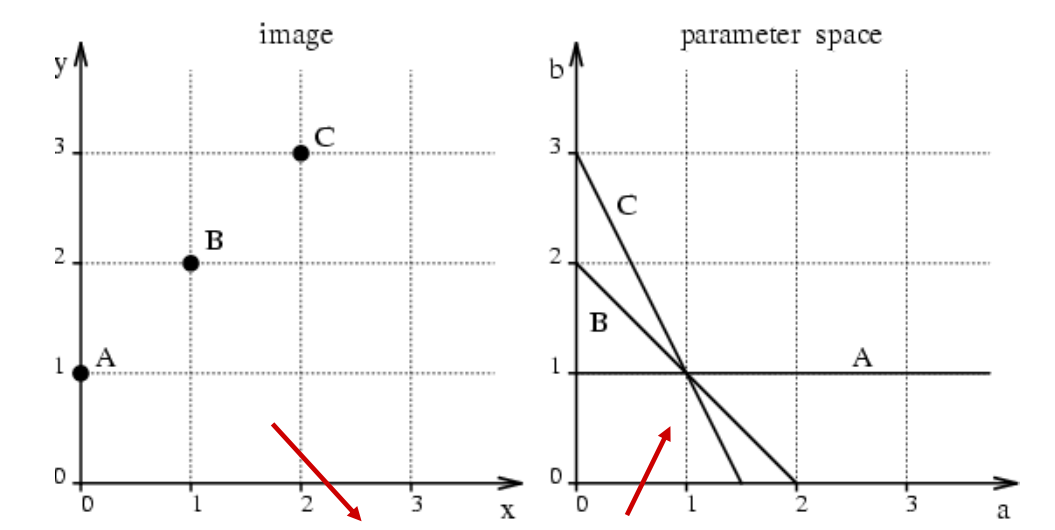
\includegraphics[width=0.8\columnwidth]{pictures/hough}

$$b = (-x)*a+y$$

Alternative: x-y space to $\theta$-$\rho$ (or d) space
$$x cos(\theta) + y sin(\theta) = \rho$$

For each point, render the curve ($\theta$, d) and count the parameter in bins with similar values.

Difficulties: How big should the bins be (too big, and we cannot distinguish between quite different lines; too small, and noise causes lines to be missed)


Hardly ever satisfactory in practice, because problems with noise and bin size defeat it

\subsection{Line fitting}
\subsubsection{Incremental line fitting}
\begin{lstlisting}[frame=single]
Put all points on a curve list, in order along the curve
Empty the line point list
Empty the line list
Until there are too few points on the curve
	Transfer first few points on the curve tot the line point list
	Fit line to line point list
	While fitted line is good enough
		Transfer the next point on the curve to tthe line point list and refit the line
	end
	Transfer last point(s) back to curve
	Refit line
	Attach line to line list
end
\end{lstlisting}  

\subsubsection{K-means}
\begin{lstlisting}[frame=single]
Hypothesize k lines (perhabps uniformly at random)
or
Hypothesize an assignment of lines to points and then fit lines using this assingment

Until convergence
	Allocate each point to the closest line
	Refit lines
end
\end{lstlisting} 

Problem can be stuck in local optima
 
\subsubsection{Probabilistic}
- EM-algorithm (expectation maximum)
- M-estimators
- RANSAC

\subsubsection{RANSAC}

- Choose a small subset uniformly at random
- Fit to that
- Anything that is close to result is signal; all others are noise
- Refit
- Do this many times and choose the best\\

\textbf{Issues} 
\begin{itemize}
	\item How many times? Often enough that we are likely to have a good line
	\item How big a subset? Smallest possible
	\item What does close mean? Depends on the problem
	\item What is a good line? One where the number of nearby points is so big it is unlikely to be all outliers
\end{itemize}


\begin{lstlisting}[frame=single]
Determine:
	n-the smallest number of points required
	k-the number of iterations required
	t-the threshold used to identify a point that fits well
	d-the number of nearby points required to assert a model fits well
Until k iterations have occured
	Draw a sample of n points from the data uniformly and at random
	Fit to that set of n points
	For each data point outside the sample
		Test the distance from the point to the line against t; if the distance from the point to the line is less than t, the point is close
	end
	If there are d or more points close to the line then there is a good fit. Refit the line using all these points.
end
Use the best fit from this collection, using the fitting error as criterium	
\end{lstlisting} 

$$ k = \frac{log(1-p)}{log(1-w^s)} $$
k - number of iterations\\
p - probability at least one sample free from outliers\\
w - fraction of inliers = d/n\\
s - model dimension (2 for a line, 3 for plane)

\subsection{Missing variable problems}

In many vision problems, if some variables were known the maximum likelihood inference problem would be easy 
\begin{itemize}
	\item fitting; if we knew which line each token came from, it would be easy to determine line parameters
	\item segmentation; if we knew the segment each pixel came from, it would be easy to determine the segment parameters
	\item fundamental matrix estimation; if we knew which feature corresponded to which, it would be easy to determine the fundamental matrix
\end{itemize}
This sort of thing happens in statistics, too - strategy:
\begin{enumerate}
	\item estimate missing variables
	\item plug these in, now estimate parameters
	\item re-estimate appropriate values for missing variables - converges to local extremum (like k-means)
\end{enumerate}

\subsection{Cross validation}
-Split data set into two pieces, fit to one, and compute negative loglikelihood on the other
-Average over multiple different splits
-Choose the model with the smallest value of this average
-The difference in averages for two different models is an estimate of the difference in KL divergence of the models from the source of the data